\begin{figure}[h]
  \centering
  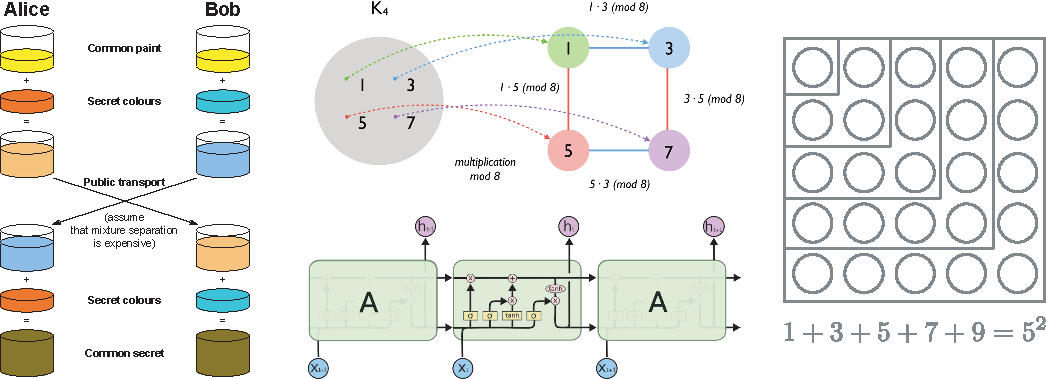
\includegraphics[width=\textwidth]{assets/interviews/teaser-a.pdf}
  \caption{
      Diagrams explain concepts visually in many domains, \eg{}: (a) Diffie-Hellman key exchange with colors representing prime multiplication~\cite{wiki:crypto}. (b) Linking two views of the Klein 4-group~\cite{OBT}. (c) Unrolling a recurrent LSTM network~\cite{UnderstandLSTM}. (d) Natural numbers as 2D areas in a visual proof~\cite{SystemsOfThought}.
  }
  \label{fig:interviews-teaser}
\end{figure}

\section{Introduction}

% Why ED is important
Visual representations of knowledge allow us to understand and disseminate information more effectively than text alone~\cite{promiseOfMultimediaLearning}. This chapter focuses on conceptual diagrams, which communicate conceptual, procedural, and metacognitive knowledge~\cite{bloomRevised} in visual form. \emph{Conceptual diagrams} (sometimes also called \emph{explanatory diagrams} or \emph{concept visualization}~\cite{conceptViz}), provide a graphical overview of conceptual models---the relationship between concrete and abstract entities~\cite{infographics}. By giving abstract concepts visual representations, these diagrams help explain concepts to oneself and communicate them with others. Explaining concepts using visuals is profoundly important for dissemination of scientific knowledge and for learning. 

% For instance, the use of diagrams in a scientific publication positively correlates with higher scientific impact~\cite{Viziometrics}. Further, creating diagrams improves learning, both when diagrams are created for others~\cite{clark2016learning}, and when they are created for self-explanation~\cite{CreatingVisualExplanationsImprovesLearning}. 


% For instance, Figure \ref{fig:teaser}d the reader that for any positive integer $n$, the sum of all positive odd numbers up to $2n-1$ is equal to \smash{$n^2$}.
% \item  Figure 1a is an instance of illustrated \emph{procedural knowledge} and Figure 1b depicts the \emph{conceptual knowledge} of Klein groups. 

% Tools for ED is too old!
% Whereas the tooling for data visualization improved significantly in the past decade~\cite{visSurvey}, tools for creating conceptual diagrams are still limited. 

While conceptual diagramming is clearly an important form of knowledge work, unfortunately, tools for creating conceptual diagrams are still limited. Current tools for diagramming of conceptual, procedural, and metacognitive knowledge~\cite{bloomRevised} stand in tension between: a) General-purpose drawing tools such as Illustrator and Figma that offer simple pen-and-canvas or box-and-arrow metaphors, but are \emph{viscous}~\cite{green_usability_1996}---users must constantly commit to exact positions, sizes, and styling of shapes. b) Dedicated diagramming tools such as Lucidchart and Gliffy that allow rapid changes, but rely heavily on templates, limiting diagrammers to a fixed set of visual representations. 

This paper argues that this relatively limited support for diagramming in tools is in part because the process of diagramming is poorly understood. For instance, often diagrammers start with informal media such as paper or whiteboards, and edit diagrams digitally before they are presented, but how do diagrammers manage the evolution of diagrams? How do diagrammers utilize the strengths and cope with the limitations of their tools? Which tools are chosen for what purposes?  Such a detailed understanding of the process can help design interactive tools to support diagramming. 

% Summary of the results
This chapter contributes a description of the process of creating conceptual diagrams, the difficulties people face while diagramming, and opportunities for tool design. These findings are based on interviews with 18 domain experts from a wide variety of disciplines such as math, computer science, architecture, and education. Our interviews reveal that diagrammers have diverse interactions with visual representations in both physical sketches and digital tools, including finding, creating, storing, and reusing representations. When diagrammers transition from sketches to digital tools, their tool selections are  influenced by their \emph{sense of control} over object placement and diagram layout. Participants were concerned with two kinds of control: local object placement, and global diagram layout. Current tools, both those that use programming languages (PL) and those that use direct manipulation (DM) as their interactive metaphor trade-off one kind of control to support the other more effectively. Consequently, we found that diagrammers invented their own set of \latin{ad hoc} and personal reuse patterns to iterate, simplify, and automate the diagramming workflow. 

One implication of our results is the opportunity to design tools informed by the processes of diagramming, and practices that domain experts already use, making digital diagramming more intuitive and efficient. We identify four key opportunities for \textbf{natural}~\cite{myers_natural_2004} diagramming tools that allow diagrammers to express their ideas visually the same way they think about them:
%
\begin{itemize} [noitemsep,topsep=-4pt,parsep=2pt,partopsep=0pt]
    \item \textit{Exploration support}: supporting exploratory behaviors such as undo and backtracking during both abstract-level, breath-first exploration of the design space and low-level refinements of visual details.
    \item \textit{Representation salience}: allowing explicit creation and management of visual representations, \ie{} the \emph{mappings} from domain constructs to shapes instead of geometric primitives themselves.
    \item \textit{Live engagement}: providing diagrammers with the sense of agency by designing for liveness and directness of the diagramming experience. 
    \item \textit{Vocabulary correspondence}: enabling diagrammers to interact with their diagrams using vocabularies that is conventional in their domain.
\end{itemize}
%
For each of the opportunities, we survey existing techniques from relevant areas to provide tool designers with technical insights on how it might be implemented.

% In short, this paper makes two contributions: first, we offer a deep, qualitative description of the process of conceptual diagramming. Second, based on the findings from this qualitative research, we propose a new framework for designing diagramming tools, \textit{natural diagramming}, describe its properties, and possible routes of implementation. 

%%%%%%%%%%%%%%%%%%%%%%%%%%%%%%%%%%%%%%%%%%%%%%%%%%%%%%%%%%%%%%%%%%%%%%%%%%%%%%%% Not used
% What ED really is and how its different from other diagrams
% Often, these conceptual diagrams are produced by domain experts that are not professional diagrammers---their diagrams are less precise than schematic drawings crafted by engineers and less ``artistic'' than paintings. These diagrams illustrate high-level ideas with just enough precision and aesthetics to be clear and illustrative. 
% \cite{designWithDiagrams}~makes a distinction between \emph{pictorial} and \emph{propositional} graphics. [some statements about the axis of abstraction for diagrams, data viz being closer to the pictorial end and concept viz being further to the propositional end:]

% However, we don't know how they are created.
% While the impact of diagramming is clear, and the general outlines of the process are well-known, a detailed understanding of the process of creating diagrams is still unexplored. As a result, tools for diagramming are designed with assumptions of what the process of creating a diagram involves.  For example, we may expect that conceptual diagrams are created on informal mediums such as paper and whiteboards to brainstorm and organize ideas, and then edited digitally for presentation in scientific publications and educational materials to communicate concepts to others. But when do diagrammers move from informal media to digital media? What difficulties do they face? And what tools might support this transition?

% Currently not used: When do diagrammers move from informal media to digital media, and what difficulties do they face?

\section{Method}

\subsubsection{Participants and recruitment} 
We conducted interviews with 18 participants (13 male, 5 female). Participants were recruited through posts on social media, and our research group website. Of these, four participants were university faculty, 10 were PhD students or postdocs, one was a professional masters student, one was a K-12 math instructor, one is an independent software developer, and one is an enterprise software engineer. Prospective participants filled out a survey which allowed us to screen participants for our interviews. We selected the interviewees based on the following criteria: the interviewee (1) creates conceptual diagrams on a frequent basis and (2) uses digital diagramming tools to create these diagrams. 

Because we had more potential interviewees than we originally envisioned (64 in all), we used a saturation method~\cite{socialResearchMethods} to determine the number of participants. We conducted several batches of interviews (with 2-3 interviews per batch consisting of diverse participants), and did a preliminary analysis of the transcripts from each batch. When the analysis stopped revealing new insights, we stopped interviewing more participants. 

\subsubsection{Semi-structured interviews}
 
Interviews lasted between 30 and 80 minutes and were semi-structured. Interviews were conducted either in person (7 participants) or online using Skype (11 participants.) We encouraged participants to bring any digital and hand drawn diagrams that they had previously created that they could share with us. We also encouraged them to have a pen and paper (or a whiteboard) available to draw during the interview. 

Four of the authors are involved in the development of \Penrose{}~\cite{DSLDI, OBT}, a new diagramming tool. Our initial interview questions were developed to inform \Penrose{}'s design. The focus of the interview eventually broadened to participants' past experience diagramming (using the critical incident technique~\cite{criticalIncident}), tool preferences, and reuse practices. The full interview protocol is included as supplementary material. Example questions from our script are: (\eg{}~ ``\textit{What is the last diagram you made?}'' and ``\textit{What is the diagram you are most proud of?}''), accompanied by appropriate follow-up questions and requests for participants to share diagrams under discussion. Table \ref{tbl:participants} includes all the participants categorized by the primary focus of their work.

\begin{center}
\begin{table}
% \begin{table}[t]
\centering
\begin{tabular}{l|l}
Domain & Participant \\ \hline
Abstract algebra & P1, P17 \\ 
Category theory & P4\\ 
Discrete mathematics & P14 \\ 
Computer graphics & P16, P6, P10, P3 \\ 
Algorithms & P12 \\ 
Topology & P7 \\ 
Human-computer interaction & P13, P18 \\ 
Programming language theory & P11 \\ 
Software engineering & P9, P2\\ 
User interface design & P5\\ 
Architecture & P8 \\ 
K-12 education & P15 \\ 
\end{tabular}
\caption{Interview participants' primary domains}
\label{tbl:participants}
\end{table}
\end{center}

\subsubsection{Analysis}
Interviews were video recorded and transcribed using either human or machine transcription. The first two authors then manually validated and corrected any transcription errors.

We employed thematic analysis methods \cite{thematicAnalysisInPsych} to analyze interview transcripts. The first two authors began by conducting an open coding session and discussed initial insights for every batch of interviews. Then, following all interviews, the authors discussed the codes and created a coding guide with operationalized definitions of codes. Using the agreed coding guide, one of the authors did a second phase of coding. While conducting the second coding phase, the author also summarized the transcripts using sticky notes containing highlights of the interview sessions. All authors then reviewed both the codebook with the sticky notes to further refine the set of codes.

Finally, the authors analyzed the codes by clustering lower-level codes during multiple interactive discussion sessions. Through the higher-level clusters, a few themes with high numbers of codes emerged, such as \emph{Reuse} and \emph{Representation}. We present these themes and the resulting insights next.

\section{Results}

% Top-level TODOs
%----------------


In this section, we present the results from our analysis of the interview data. The section is organized in terms of the high-level themes that emerged from our analysis.

\subsection{Representation finding}

When illustrating a concept visually, a crucial step is to decide how every abstract object will be represented graphically. For example, Larkin and Simon, in their classic paper ``Why a Diagram is (Sometimes) Worth Ten Thousand Words,'' chose to represent forces with arrows in the diagram shown in Figure~\ref{fig:forcediagram}b~\cite{whyDiagramWorth}. This step, which we call \textit{representation finding}, is crucial to diagram effectiveness. If Larkin and Simon had represented forces using concentric circles with different radii instead of arrows (Figure~\ref{fig:forcediagram}c), the directionality of the forces would be lost. If they had represented forces with chocolate bars with different lengths (Figure~\ref{fig:forcediagram}d), the diagram would have been inconsistent with other physics diagrams and the extraneous detail would have distracted from the core purpose. 

\begin{figure}
    \centering
    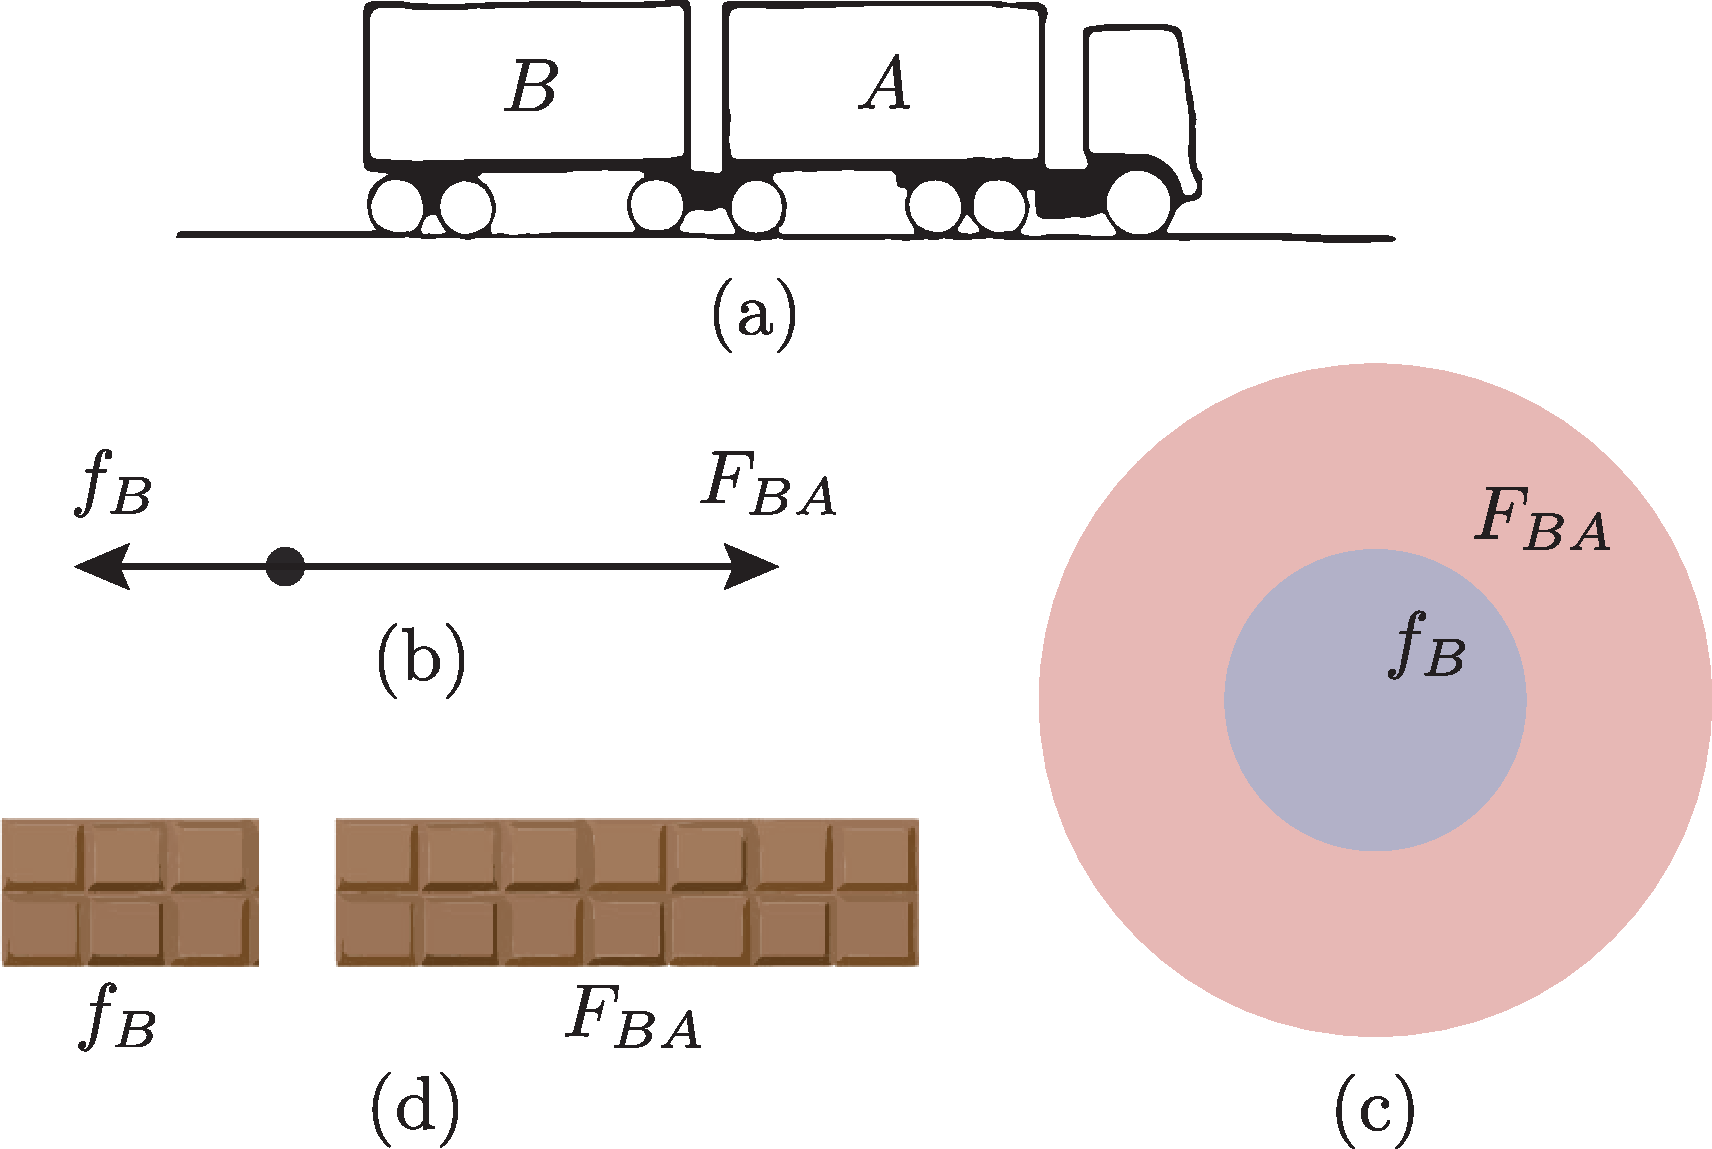
\includegraphics[width=8cm]{assets/interviews/larkin-simon-labeled.pdf}
    \caption{A good visual representation (b) of forces on a truck (a) is easily understandable, whereas (c) loses essential information and (d) is non-standard and harder to understand.}
    \label{fig:forcediagram}
\end{figure}

This process of \textit{representation finding} usually preceded the creation of any formal or informal diagrams. Participants engaged in two representation finding activities: (1) seeking and finding existing representations from prior work and (2) creating novel representations. 

\subsubsection{Diagrammers seek existing representations from prior work}
In many domains, there are well-established visual representations for abstract concepts and objects. Therefore, diagrammers tended to look at existing diagrams for  representations when starting to create their representations:

\itquote {Sometimes I look for inspiration in other papers just to know what kinds of standard people are using. Sometimes there are some conventions that people actually use in my field like how to represent a camera for instance. So you kind of have to stick with these conventions.} (P3)

\subsubsection{Diagrammers generate new representations to tell new stories} 
Other domains lack standardized representations and diagrammers creatively \textit{generate} their own representations:

    \itquote{The whole purpose of those diagrams [in my book] is to make something that has never been seen before visually obvious... Why didn't anybody draw that picture before? I have been taking something that almost seems completely confusing or unimportant and having a picture that makes you know what's going on... is truly satisfying.} (P1)

When creating diagrams for explanatory purposes, diagrammers also carefully craft visual representations to ensure that the diagram is intuitive and clear for their target audience. For instance, P8 developed new representations to reduce visual complexity:
    
    \itquote{When a diagram has too many working elements, it becomes too hard for your brain to process it. If you can boil it down to two main things interacting, that will make the diagram much more intuitive to someone. It's very much about choosing the right colors, lines... putting the emphasis in the right place.} (P8)

\subsubsection{Diagrammers use sketches to discover appropriate representations}

Sketching plays an important role in generating new visual representations or choosing among existing ones. For instance, P8, P12, P5, P9, and P13 reported iterative processes of refining their visual representations as they sketch. For instance, P9 described the evolution of diagram sketches and the changes of visual representations of the design of a complex camera-supporter-projector system, also shown in Figure~\ref{fig:sketch}:

    \itquote{At this stage, I don't even know how these machines would be connected, so there's lines, but at this later stage I was actually thinking about `Oh, how are we going to represent these things and compute with them in practice?' So I did arrows. There's also certainly increased complexity in the beginning thing, I'm just looking at the situation of a single camera projectors supporters system. Then here on the next page I'm starting to look at different configurations of multiple cameras and projectors.} (P9)

\begin{figure*}
     \centering
     \begin{minipage}[c]{0.49\textwidth}
         \centering
         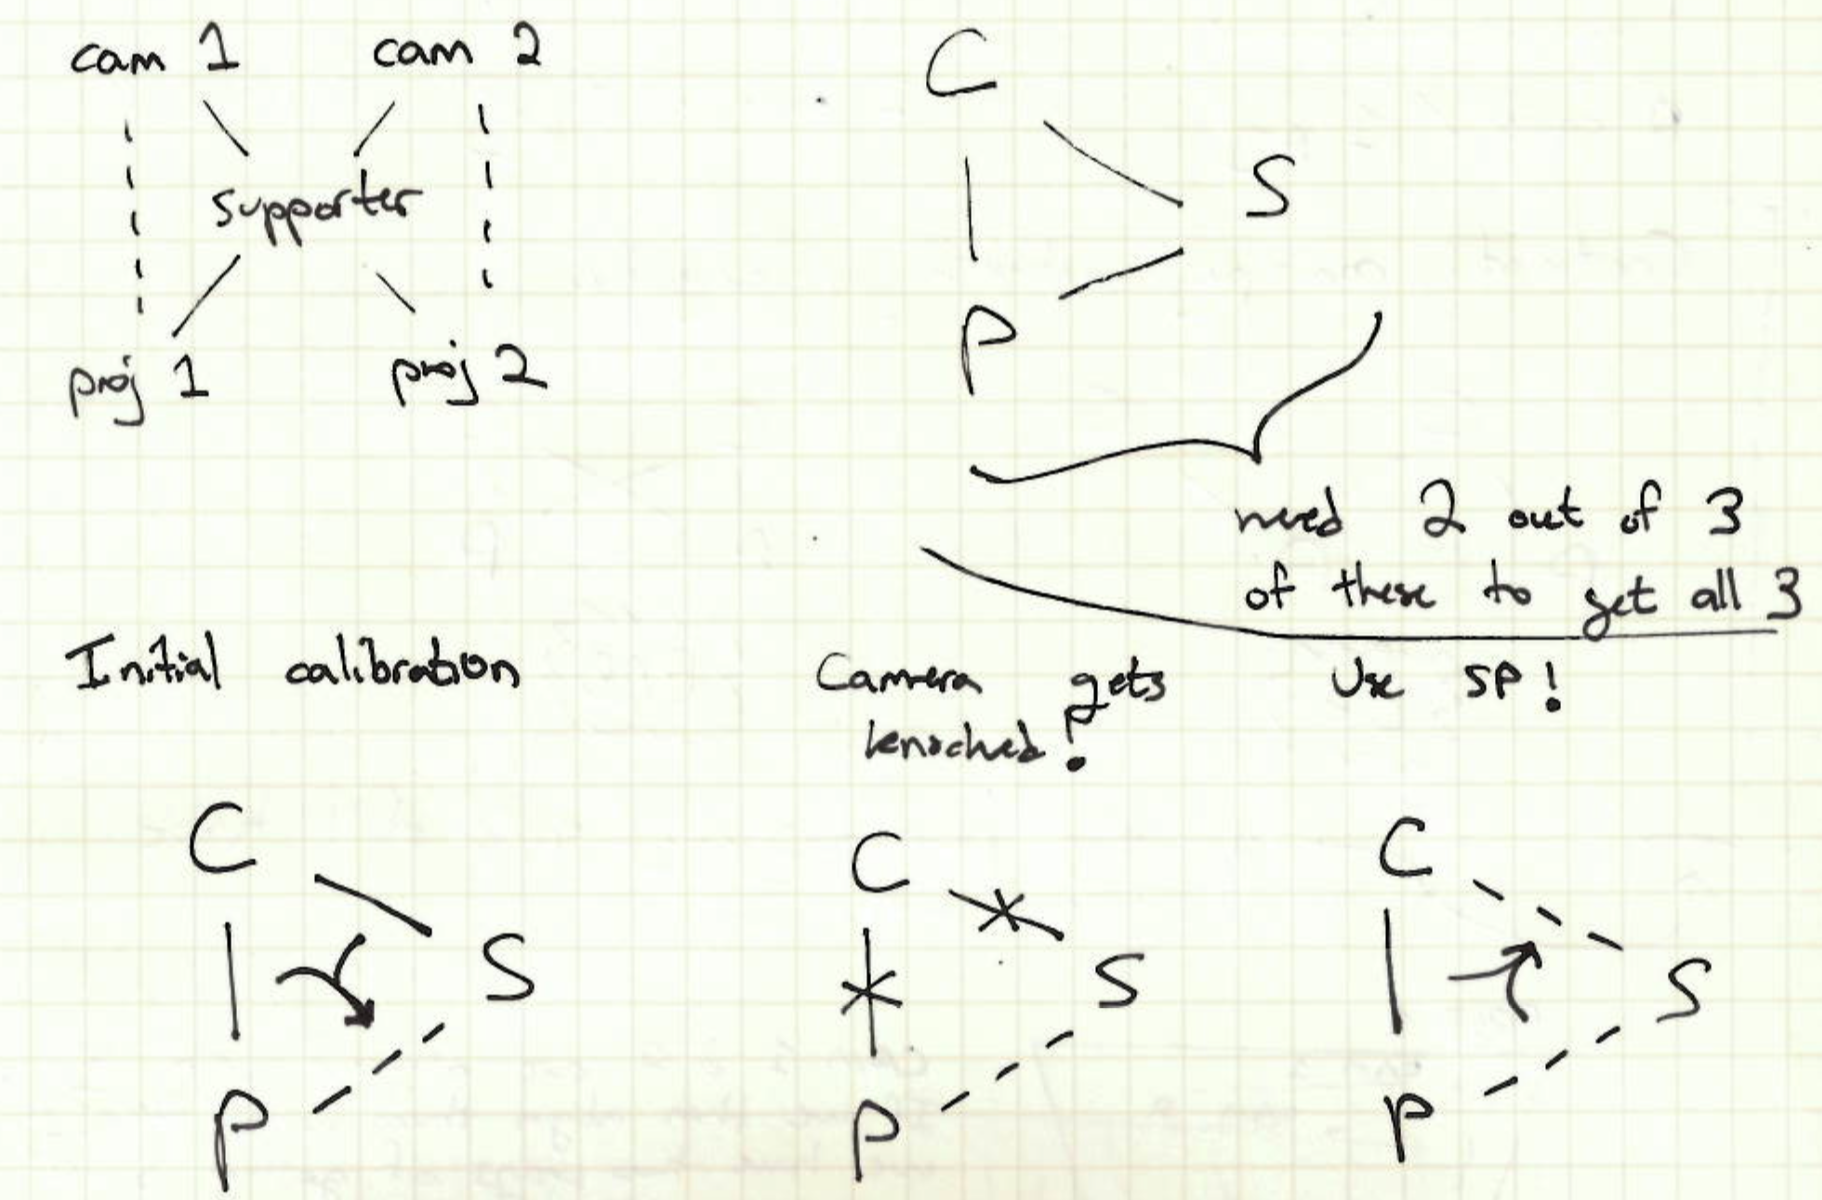
\includegraphics[height=5.5cm]{assets/interviews/sketch-1.png}
         \label{fig:sketch-1}
     \end{minipage}
     \hfill
     \begin{minipage}[c]{0.49\textwidth}
         \centering
         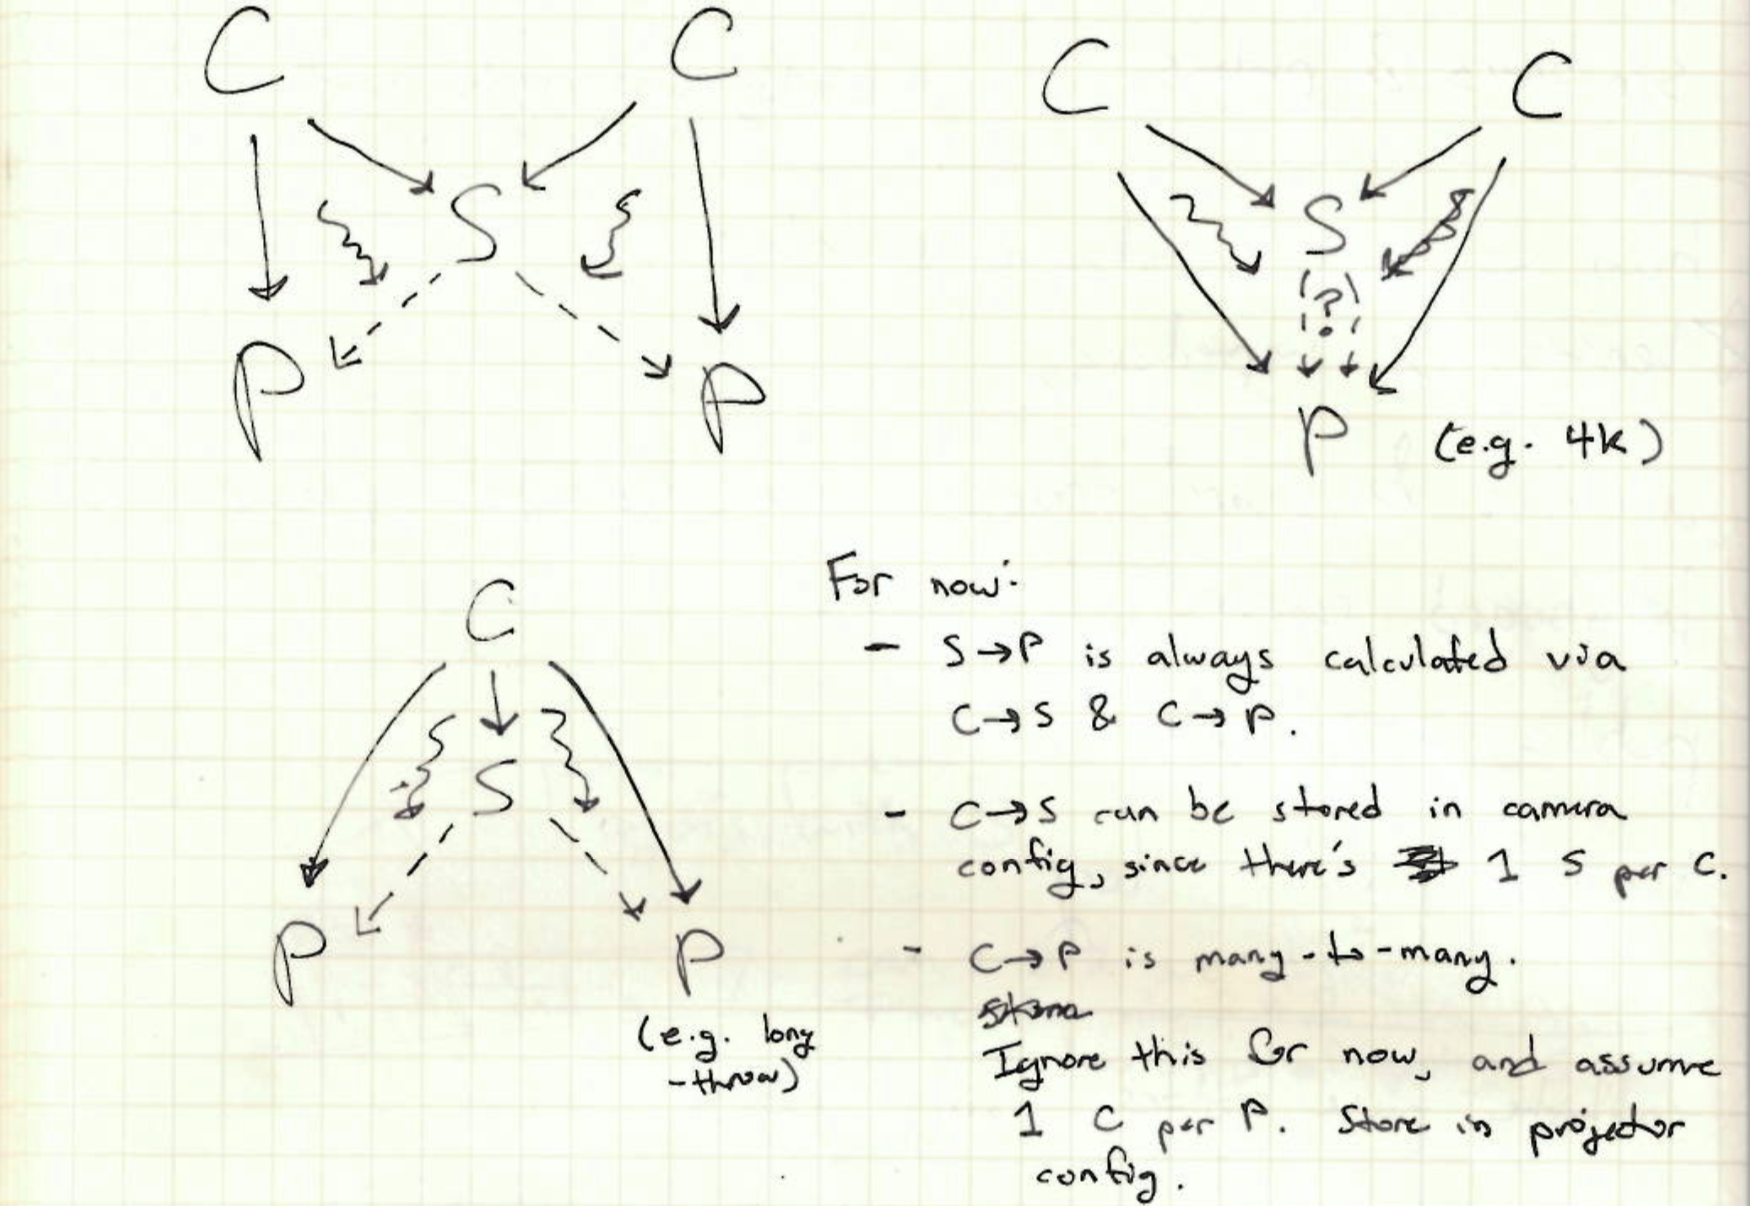
\includegraphics[height=5.5cm]{assets/interviews/sketch-2.png}
         \label{fig:sketch-2}
     \end{minipage}
     \caption{P9 made sketches to explain projector and camera calibration. The complexity of these sketches increased and visual representations evolve over time. \figloc{Left}: an initial sketch represents connectivity as line segments. \figloc{Right}: a later sketch represent connectivity as arrows. }
     \label{fig:sketch}
\end{figure*}

\subsection{Choosing the right tools} 

When participants eventually chose to move to a digital medium, their choice of tool was systematic, if not conscious. Specifically, we found participants' preferred either  programming-language based (PL) tools or  direct-manipulation based (DM) ones. Below, we analyze the reasons for their preferences. 
    
\subsubsection{People choose DM tools for faster feedback and global control}
DM tools were often described as ``easier'' and thus have lower barriers to entry when compared with PL tools.  One particularly common reason for choosing DM tools was the need to place shapes in relations with other shapes, which is difficult to do without immediate visual feedback.

    \itquote{So I like [a DM tool] because it gives me this very fine control over how things are aligned and when they're straight up and down.} (P2)
    
Because of the synchronized visual preview, DM tools provide better support for \emph{global} control over diagram layout, i.e. the relationships among graphical primitives. Diagrammers used DM tools similar to how they used pen and paper, to offload their working memory~\cite{whyDiagramWorth}, but with the additional benefits provided by interactions supported by the tools:

 \itquote{I'm trying to draw things down on the papers [or DM tools] because my head is getting crowded and I need to be able to keep track of everything on [digital] paper and be able to interact with it the same way I would in my head.} (P7)

\subsubsection{People choose programming languages for better abstraction and local control}

Comparing to the easy \emph{global} control provided by DM tools, PL tools make \textit{local} control easier: they let users control \emph{local} placements of shapes by specifying exact pixel coordinates:

    \itquote{I want this [a shape] to be exactly a hundred pixels... because there's definitely times where I want to get this right to this point and it's hard to do that with the mouse.} (P15)

Global layout of diagrams can be specified more precisely using PL tools, but requires more advanced programming skills and, as discussed, more time commitment:

    \itquote{If it's something where the relationships among the things you want to specify in a precise way, then it's a lot easier, if you know how to program, to introduce a programming language where you can specify exactly the relationships you want, how you want them to change, and so forth.} (P1)

Programming languages provide affordances to create abstractions and automate the diagramming process:

    \itquote{Once you have made a visualization [using PL tools], if you want to tweak things about it, you can. Just put what you do into a script, add some parameters, and you could repeatedly get the same visualization with variations... It will generate the thing automatically, you don't have to create a whole picture by hand again.} (P1)

The complexity of languages, however, incurs a higher upfront cost and steep learning curve, making more diagrammers without programming background reluctant to commit to them. Another downside of PL tools is that they often require compile-and-run cycles and hence delayed feedback:

    \itquote{There's a long learning curve on [a PL tool] and then it's slow. It's a lot of typing and a lot of iterative--`I type something and I see what it looks like'. So there's a lot of delays in modifying [the diagram].} (P15)
    
    \itquote{I'm willing to put in the effort, but it's like 20\% of the time is that, and like 80\% of the time is fighting with \LaTeX.} (P11)

\subsubsection{Advanced diagrammers use PL tools to automate their diagramming workflows}
In some cases, diagrammers find the need to create families of similar diagrams for the use of, for instance, writing a textbook or a problem set. A small number of our interviewees automated their diagramming workflow extensively by leveraging the abstraction affordances of PL tools. One automation pattern is to parameterize complex diagrams and generate multiple instances with variations to explore design alternatives and populate diagram collections:

    \itquote{If I invest the time upfront to just write it, parameterized by, and then I do the diagram in terms of $n$ and $k$. And then later I realize that, `Aw, $n=15$ and $k=4$ is just a mess!' Okay, I go to the top of the file and I set $n=12$ and $k=3$ and I re-render it and it looks like this, and I go, `That's what I want.' If I'm not sure, okay, let's try $n=10$, try that. You can just make a new diagram in 15 seconds instead of four hours, but they also demand more time and skills up front. If I'm just going to do one diagram, it's not worth it.} (P1)

Another pattern is creating \latin{ad hoc}, embedded domain-specific languages that allow specification of diagrams at a higher level:

    \itquote{I have learned a style that is highly idiomatic and not something that I could teach someone else... you look at the sort of syntactic objects that you're going to work with in a certain proof theory, and you define the macros at the top level.} (P11)
 
As commented by P1 and P11 above, the automation requires a high upfront cost and advanced skill sets, and only advanced diagrammers invested in the skills and time commitment to do so.


% TODO: move this conclusion to somewhere else
% As a result, PL tools are preferable when multiple diagrams with common, repeated elements are needed, whereas DM tools are more suitable for creating a single diagram. However, DM tools require low-level manipulation of geometries and thus more manual workflows.

\subsection{Reusing elements from earlier diagrams}

\subsubsection{Diagrammers backtrack frequently and informally track prior versions}
Diagrammers were iterative even in the formal diagramming stage, which involves frequent backtracking behaviors. Therefore, keeping track of version history becomes an essential task for diagrammers. 

In the case of DM tools, however, versioning can be challenging in many existing tools, due to the lack of textual storage formats. As a result, \latin{ad hoc} solutions are again created to compensate for this limitation such as keeping multiple versions of the diagram on the same canvas, as illustrated in Figure \ref{fig:multiple} and described by P5: 

    \itquote{I ... duplicate each [art board], change something about that, and take it out again. That's really helpful not only to present the overall trajectory of the process, but then you can go back and reference a previous state without having to look through the undo history and destroy all of your redos. I [like to] branch out fractally with different areas that are relevant to me.} (P5) 

\begin{figure*}[t]
% \begin{figure*}
    \centering
    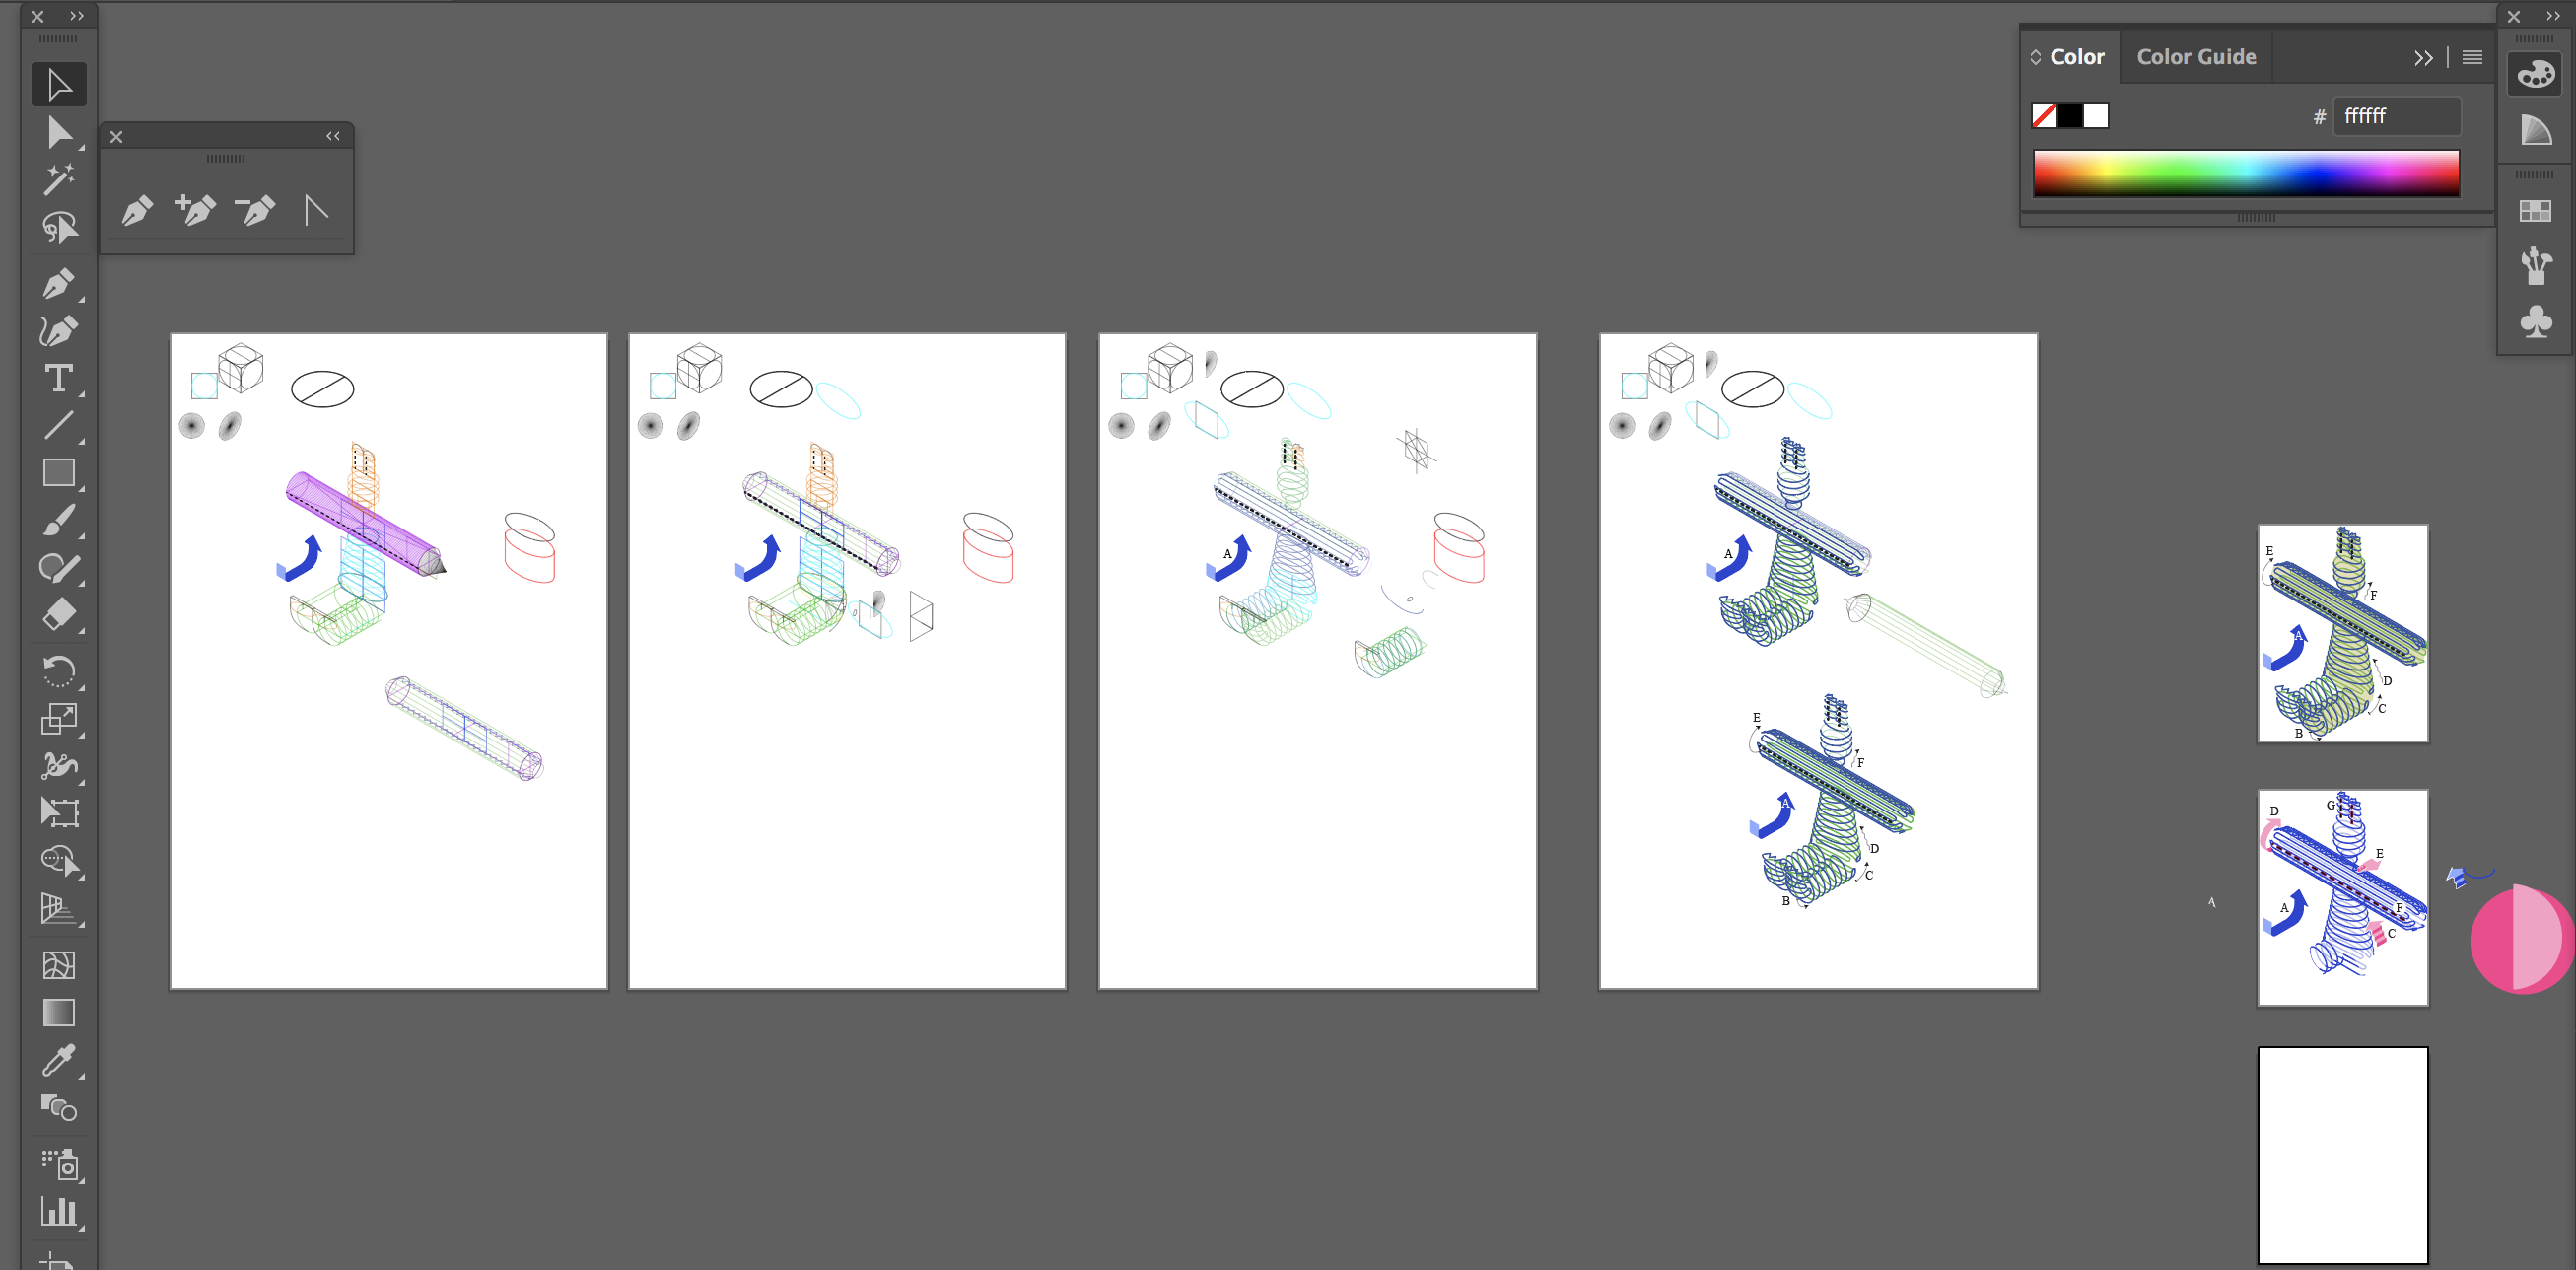
\includegraphics[width=15cm]{assets/interviews/MultipleCanvases.png}
    \caption{P13 manually tracks versions of a diagram in Illustrator using multiple canvases.}
    \label{fig:multiple}
\end{figure*}

In theory, standard version control systems such as \texttt{git} \cite{git} make it easy to track versions with PL tools. However, even with their textual file formats, versioning can still be challenging for PL tools because textual representations of diagrams can be too low-level to be human readable. As a result, P6 tracks prior versions without using standard version control systems:
    
    \itquote{I rely either on Dropbox to store different images or I have my own custom-made back-up system that keeps hard copies of things... I have a separate script that every day pulls all of my folders and keeps copies of them if there is any change.} (P6)
    

\begin{figure}[ht]
    \centering
    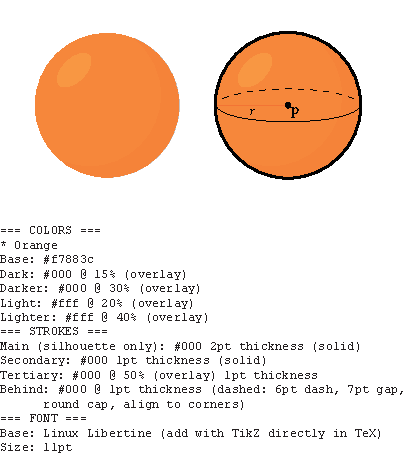
\includegraphics[width=7cm]{assets/interviews/cheatsheet.pdf}
    \caption{P3 uses a cheat sheet to track frequently used style attributes.}
    \label{fig:cheatsheet}
\end{figure}
    
\subsubsection{Diagrammers organize reuse libraries by representation}

The most common form of library we saw diagrammers maintain was a ``cheat sheet''. Cheat sheets are configuration files that contain low-level parameters such as line-weight settings and hexadecimal strings of colors (P3, P6, P13). Diagrammers used cheat sheets to reduce stylistic inconsistencies and to simplify the repetitive, manual tasks in the diagramming process with cheat sheets.  For instance, one participant said: 

    \itquote{Usually I have this little \texttt{txt} file where I basically remember the color so I have the color codes for primary and secondary [objects]... I saved the [line] width as well for primary secondary [objects], and that's kind of like my cheat sheet that I reuse.} (P3)
    
This is one area where tool support was mostly lacking. For instance, participants often took notes manually (sometimes these notes were handwritten.)

\begin{figure*}[t]
% \begin{figure*}
    \centering
    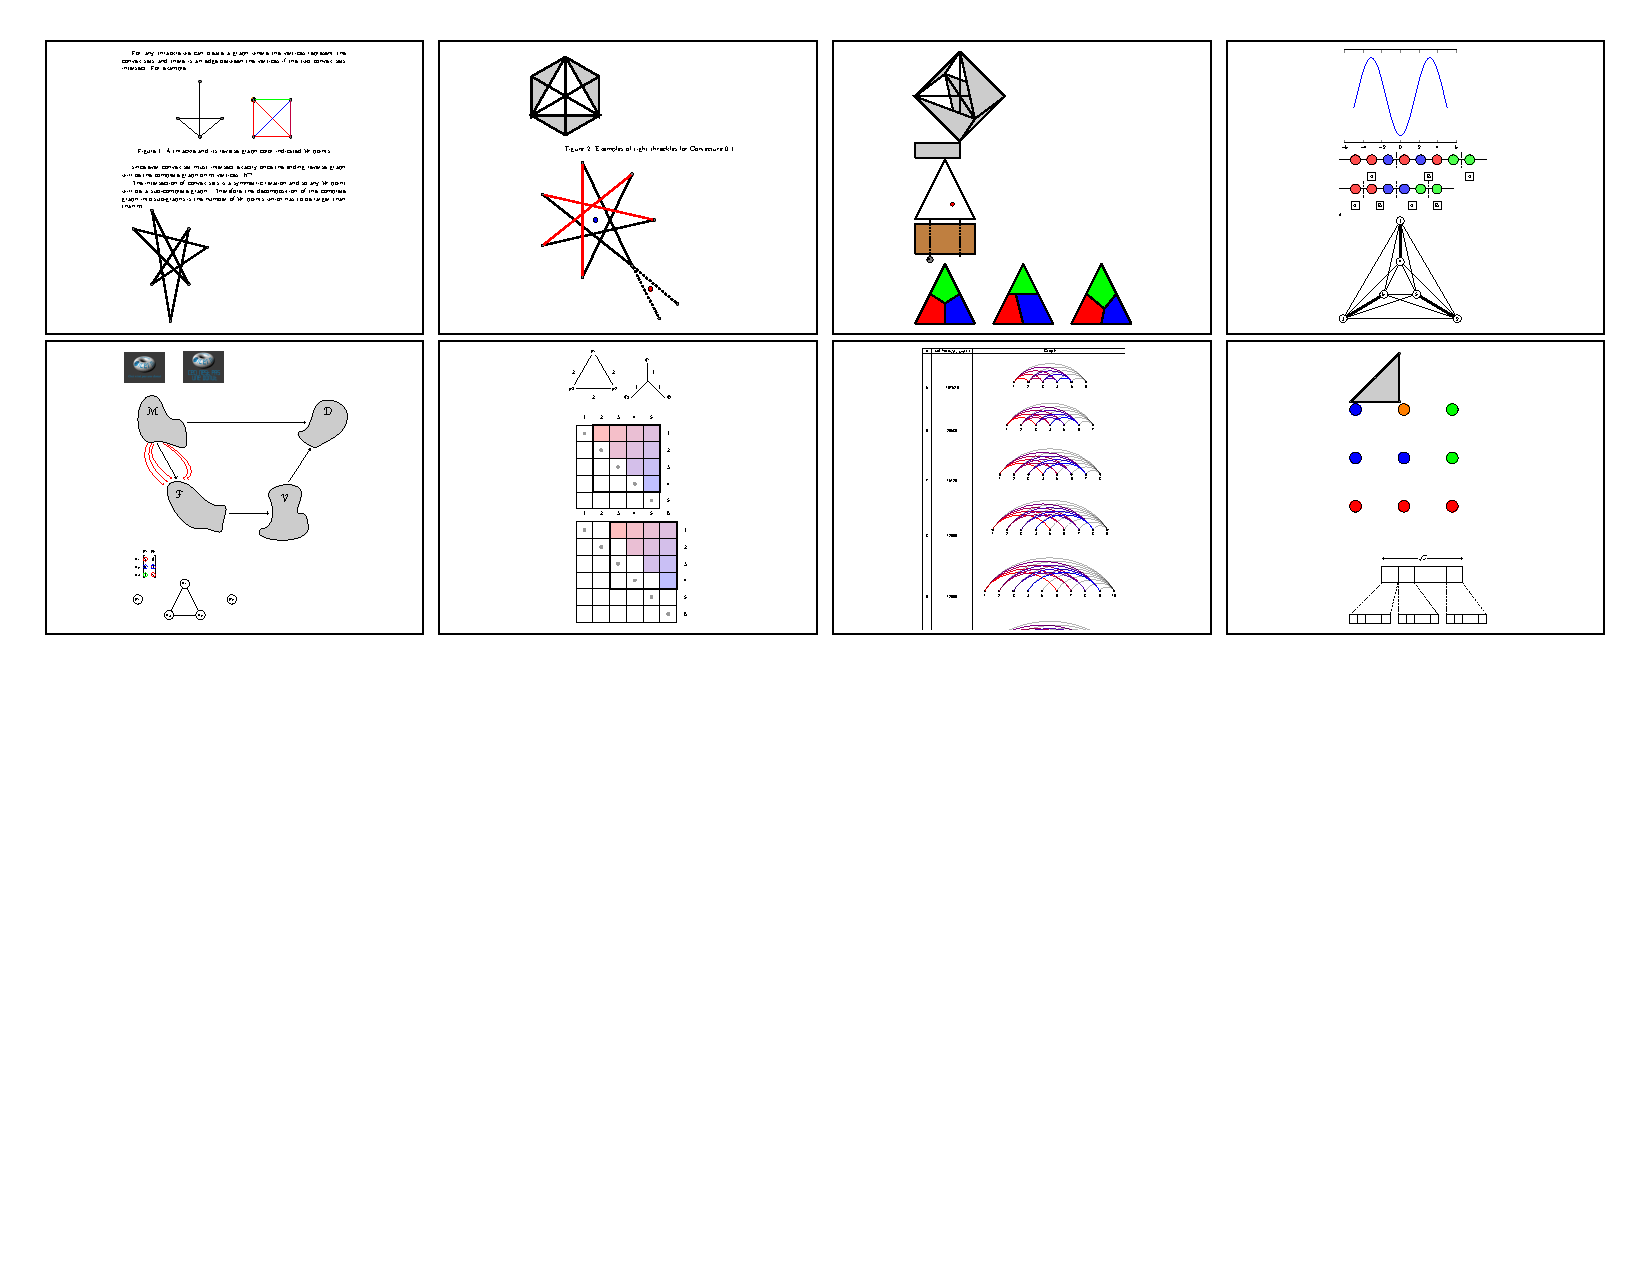
\includegraphics[width=15cm]{assets/interviews/library-cropped.pdf}
    \caption{P7 organizes all previously made TikZ diagrams in a single document.}
    \label{fig:library}
\end{figure*}

More advanced diagrammers maintained collections of existing diagrams or diagram components, organized by representation. For instance, one participant keeps a document of previous visualizations, as shown in Figure~\ref{fig:library}: 

    \itquote{I keep a document, that is almost all the TikZ diagrams I've ever had to because I find that they helped me think about how to represent diagrams for new situations.} (P7)

Another participant collects commonly used diagram components in a personal library:

    \itquote{So over the time I've settled on specific representations for the camera and the light source, I keep copies of them. I have my own small library of things.} (P6)

    
%%%%%%%%%%%%%%%%%%%%%%%%%%%%%%%%%%%%%%%%%%%%%%%%%%%%%%%%%%%%%%%%%%%%%%%%%%%%%%%% Unused sections

% \subsection{Sketching}

% 16 of 18 of our participants use sketches to ideate and prepare for formal diagrams. Our findings about sketches are mostly in line with the conventional wisdom and existing literature: (1) sketches are low-cost, low-commitment models that can be used for rapid iterations and (2) the low fidelity of sketches often make them a transitional step in diagramming, before going into digital tools. 

% \subsubsection{Sketches as low-cost, low-commitment representations}
%  Among 18 participants, 16 of them reported that they use sketches to ideate and prepare for formal diagrams.

% Because they have lower fidelity, they require less effort to compose and thus is more tentative. According to our interviewees, a sketch ``doesn't have to be perfect''  and ``is just the intent and placement of things in the diagram'' (P3). The informality of sketches enables a lower level of commitment and lack of finality, 

%     \itquote{In the process leading up to making the actual diagram, I would start with some sketching like hand and paper, just to know what I would like to do. In fact, just about every illustration that I made, I would sketch out a quick scribble out on paper.} (P1)

% Furthermore, diagrammers generally did not share sketches with others, but rather kept them as a personal collection of ideas or reference material for making formal diagrams later in the process. 
% \subsubsection{Diagrammers stop sketching when they can benefit from computational tools}

% Due to the limited complexity and lower fidelity, sketches can become unreadable as the diagram evolves to a more complicated form: 

%     \itquote{I just threw stuff together really quickly in Microsoft Word... But then, it turned out to be complicated enough that my bad diagrams weren't helpful. So I was like `okay, I better create a better version'. So, I had to go back and do it properly.} (P1)
    
% In addition, the lower fidelity of sketches also precludes using them for certain inferential tasks. For example, diagrammatic proofs require a certain level of fidelity for one to evaluate their correctness, as one participant said:

%     \itquote{I don't feel like I really understand whether or not I've done the thing correctly until I really have a [formal] diagram that I can look at and feel confident about.} (P11)

% Even when used for inferences and proofs, diagrammers avoid the overhead of digital tools in early stages of diagramming as they plan out the diagram. Therefore, many of them prefer to plan with sketches and move on to digital tools once they can fully leverage the power of the tools, as participant P11 from above said:

%     \itquote{There might be small errors [in a draft] that I need to fix, but in a process of creating the sort of final draft, I'll find them. So I know that about myself, so I'm willing to put in the effort.} (P11)
%     % \itquote{I'm willing to put in the effort, but it's like 20\% of the time is that, and like 80\% of the time is fighting with LaTeX.} (P11)
    
% As tools, pen and paper afford a unique sense of freedom and control, as one participant describes:

% \itquote{It just feels like an extension of my own brain and my own hand. It doesn't feel like an alien object that I'm working on, but rather it just feels like it's a part of me.} (P8)

% When using more simplistic tools like pen and paper, diagrammers are more confidant and  in \textbf{control}. Therefore, many diagrammers will not convert sketches to digital tools easily unless they have to: 

%     \itquote{I would only try to actually make it on a computer if I knew I needed to put it in the paper.} (P12)
    
%     \itquote{I don't have mastery of any computer drawing tools... I don't use [computer tools] as a matter of habit... I think of using them mainly in situations of communication, situations where I actually want to prepare something to show something in a presentation or put in a big poster or something like that.} (P9)


\section{Implications: Natural Diagramming}

The results discussed above suggest unique strengths and weaknesses of existing PL and DM diagramming tools. This section offers some possibilities to combine the strengths of PL and DM tools and create more intuitive and efficient next-generation tools. Just as previous work advocated for creating programming tools ``for people to express their ideas in the same way they think about them''~\cite{myers_natural_2004} as an opportunity for \emph{natural programming}, we advocate for creating diagramming tools for \textbf{natural diagramming}. Natural diagramming presents four distinct opportunities to leverage the strengths while alleviating the weaknesses of existing tools: exploration support, representation salience, live engagement, and vocabulary correspondence. We end the description of each of these natural diagramming opportunities by highlighting existing techniques that may be further developed to achieve it. 

\subsection{Exploration support}

Exploration pervades the diagramming process for making conceptual diagrams, from choosing representation to determining stylistic details. We characterize two types of exploratory activities by adopting terms from Goel~\cite{sketchesOfThought}: (a) \emph{Lateral transformations} involve ideation and exploration at the high-level to broaden the design space, \eg{} finding the appropriate visual representation for forces in Figure~\ref{fig:forcediagram}. (b) \emph{Vertical transformations} 
 are more detailed refinements to a pre-determined visual representation, such as deciding the arrowhead style in Figure~\ref{fig:forcediagram}b.

Sketching is an important, if not necessary, part of the design process~\cite{BuxtonBook}. Our participants produced physical sketches to explore design alternatives before transitioning to digital tools, which are perceived as a medium of higher commitment. They performed this type of exploration by looking at prior work and multiple alternatives \emph{laterally}. Early informal sketches naturally affords lateral transformations~\cite{sketchesOfThought}. 

Diagrammers also attempt to leverage precision, automation, and abstraction afforded by digital tools. After the visual representation stabilizes, they move to digital tools and refine this determinate representation, i.e. \emph{vertically} refine their design. Unfortunately, existing tools do not provide sufficient flexibility to support even small vertical changes. Whereas DM tools require significant manual efforts to propagate local changes, PL tools require a high upfront cost to create abstractions that reduce future repetition. As a result, our participants described various \latin{ad hoc}~workarounds to perform common activities for exploration such as backtracking, versioning, and reuse in both PL and DM tools. 

In essence, a gap exists between \emph{drafting} and \emph{crafting}, a design dilemma that has plagued other sketching tools (such as digital pens)~\cite{AsWeMayInk}. Solving this dilemma requires tools that continuously support diagrammers to explore lateral and vertical changes, allowing more fluidity to make, track, and revert changes.

% Howto

One solution to the problem of exploration and change management can be seen in tools for exploratory programming. \emph{Exploratory Programming} (EP) characterizes a practice of experimenting and prototyping adopted by programmers across a wide range of domains~\cite{EP-Original,exploringEP}. Data scientists reuse and iterate on small snippets of scripts to analyze data exploratively. \textsc{Variolite}~\cite{Variolite} support local versioning with ``variant boxes'' around regions of code. Software engineers often backtrack by manually deleting or re-typing code when developing software~\cite{backtrackingLongitudinal}. \textit{Selective undo} techniques allow complex backtracking in code editing~\cite{yoon_supporting_2015}, which was also shown to be effective for painting applications~\cite{myers_selective_2015}. 

Some systems also show opportunities for automatic vertical refinement. For instance, to support the transition from freehand sketches to final UI implementation, \textsc{SILK} recognizes hand-drawn shapes and translates them to real UI components~\cite{InteractiveSketchingUI}. \textsc{DreamSketch} generates 3D models from sketches~\cite{DreamSketch}. Sketches for conceptual diagrams, however, can often be intentionally ambiguous and unstructured, making recognition, beautification, and generation of reusable diagram components challenging~\cite{designSketches}.

Finally, in addition to better support for history management, another approach may be to reduce unnecessary changes through improved abstractions. \emph{Program synthesis} can be used to generate reusable functions from examples of lower-level interactions with a potentially non-programmatic interface~\cite{programSynthesis}. \textsc{Sketch-n-Sketch} is a vector drawing tool with synchronized code and graphical views of the same drawing~\cite{Sketch-n-Sketch}. It synthesizes reusable functions from direct manipulation of objects in the graphical view and thereby enables users to avoid repetition. \citet{Kevin-NIPS} synthesize imperative programs from hand-drawn sketches. Currently, synthesizing high-level abstractions and surfacing them in a non-obstructive, meaningful manner are still open problems for future conceptual diagramming tools.

% TODO: \textsc{lillicon}~\cite{lillicon} infers multiple representations of the same grayscale vector graphics.

\subsection{Representation salience}

% Intro
Constructing and interpreting representations are crucial skills for learning new concepts and developing domain expertise~\cite{ainsworth_drawing_2011}. Many of our participants track prior representations, curate reuse libraries, search for ones created by others, and inventively create new ones in their \emph{representation finding} phase. This suggests an opportunity for natural diagramming tools that support \textbf{representation salience}, treating visual representations as first-class entities and providing operations to easily interact with them. 

% Connection with the results
Bret Victor uses the analogy of climbing ``up'' (\emph{abstraction}) and ``down'' (\emph{concretization}) the \emph{ladder of abstraction} to characterize the process of understanding complex systems using visual representations~\cite{ladderOfAbstraction}. Abstraction and parametrization of diagrams allows fast generation of families of similar diagrams, which can be used in multiple places or serve as a set of design alternatives. In existing tools without easy access to abstraction constructs, generating design alternatives can be a time-consuming  manual process. Our participants use existing abstraction constructs such as macros and functions to encode representations, but they tend to be highly personalized and brittle solutions. As a result, these custom abstractions are rarely scalable or composable, as one frequent TikZ user said \textit{``macros are terrible, [I make macros that are] 20 or 30 braces deep... it's just hard to write and edit.''} (P11) In addition, these poor abstractions still require significant time investment and force diagrammers to concretize concepts manually instead. Consequently, diagrammers' representational encodings are scattered in manually curated personal libraries, online examples, and cheatsheets of lower-level elements.

% Problem statement
For visual representation to be \emph{salient}, both the underlying structures and mappings to visual elements need to be encoded in the diagramming system explicitly. Further, these encodings must be specified with \emph{manageable, scalable, and composable abstraction constructs} that allow diagrammers to move ``up'' and ``down'' the ladder of abstraction easily.

% Howto
The management of visual representations at different levels of abstraction can be seen in many fields. For instance, Gross \cite{cocktailNapkins}~tackles the problem of the fixed low-level representations of computer-aided design (CAD) tool by supporting gradual transition from sketches to more structured diagrams and suggesting concrete representations given early conceptual sketches. Data visualization tools such as Dashiki~\cite{dashiki} and Draco~\cite{Draco} can manage of multiple representations of the underlying data. 

The lack of representation salience often manifest in highly \emph{viscous} diagramming tools that operate on low-level primitives and lose deeper \emph{semantics} of graphical components. To solve this problem in data visualization, the \emph{grammar of graphics}~\cite{wilkinson_grammar_2012} formalizes a rich set of operations to transform data into visual components. For mathematical diagrams, \textsc{Penrose}~\cite{DSLDI} includes two domain-specific languages that decouple visual representations from declaration of abstract objects and encode visual representations by pattern-matching on the objects and declaring visual elements. Apart from these domain-specific solutions above, however, conceptual diagramming tools still lack a general and accessible approach to specify problem domains and the visual representations thereof. 

\subsection{Live Engagement}

% Intro & Connection with results
\citet{DM-Seminal} introduce \emph{direct engagement}, ``the \emph{qualitative} feeling that one is directly engaged with \emph{control} of the objects,'' as an important criterion for effective interfaces. Our results show that direct engagement for diagramming can be perceived differently depending on the kinds of interfaces and the sense of \emph{control} they afford, \ie{} the sense of agency over essential operations in conceptual diagramming~\cite{senseOfAgency}. DM tool design affords continuous representations of objects and immediate visibility of incremental changes~\cite{DirectManipulation-Shneiderman}. As a result, they naturally afford a sense of \emph{global} control over the global rearrangement of diagram layout. Yet, \emph{local} control over precise specification of visual properties and creation of high-level abstractions is still challenging in direct-manipulation tools. On the other hand, while these same operations are directly supported in PL tools, our participants reported frustration with their high latency and long compile-and-run cycles. Our results suggest immediate visual feedback (or \textit{liveness}~\cite{Viva-Liveness}) is also essential for abstract operations. In other words, the sense of control and direct engagement is diffused among DM and PL tools.

% Problem statement
% Taken together, these findings reflect (a) diffusion of direct engagement and the sense of control among DM and PL tools and (b) a tension between abstraction and liveness. How can we \emph{bridge the gap between DM and PL and provide full control over diagram elements}? How can we \emph{augment direct interactions with automation without sacrificing liveness completely}, as current PL tools do? 

% Howto
Traditional direct manipulation interfaces can be augmented by novel interaction and programming techniques such as programmatic brushes~\cite{dynamicBrushes}, \emph{programming by example}~\cite{PBEExcel} and \emph{programming by manipulation}~\cite{PBMLayout}. \emph{Bidirectional programming}~\cite{prodirectVision} proposes to combine direct manipulation and textual programming by surfacing both direct manipulation and text-based interfaces and synchronizes and synchronizing changes in both directions: (i)~from the program text to the output (liveness) and (ii)~from the output to the program text (direct engagement). These techniques, although currently limited to narrower domains, provide promising directions towards bridging the gap between PL and DM tools.

There have been also significant advances in programming languages to support liveness. \emph{Live programming} techniques can provide responsive and continuous feedback on program changes. The methodology has been increasingly adopted in computer science education, web development, and traditional programming environments~\cite{mcdirmid_living_2007, wysiwyc, SEEDE}. Tanimoto~\cite{Viva-Liveness} proposes four levels of liveness with the top level featuring ``stream-driven updates'' and ``informative, significant, responsive and live'' visual representations of programs' dynamic behaviors. Techniques such as incremental compilation and type inference~\cite{mcdirmid_superglue_2006} and typed holes~\cite{typedHoles} allow fast compilation and facilitate liveness of programming environments. However, many live programming systems only offer one-way updates from the program to its output visual representation, inhibiting the opportunities for direct interactions with the visuals.

\subsection{Vocabulary correspondence}

% Intro
Conceptual diagrams are made of ``abstract and topological''~\cite{designingWithDiagrams} shapes that are mapped from domain objects in the \emph{content model}~\cite{fundamentalDesignVars}. In Figure \ref{fig:forcediagram}b, the concept of two counteracting forces (domain objects) is mapped to two arrows, but the exact styling and lengths of the arrows do not change the meaning of the diagram. As a result, users' vocabularies for conceptual diagramming are often abstract, topological, and domain-specific. Therefore, there is an opportunity for natural diagramming tools that support \textbf{vocabulary correspondence} by having a grammar or an interface that directly maps to users' vocabulary for diagramming. 

% Connection to results
As shown in our results, diagrammers define new abstractions to both automate and \emph{naturalize} their diagramming process. More advanced diagrammers create abstractions to quickly generate new diagram instances and fit their mental models, but, even for advanced diagrammers, abstractions are brittle and often not share-able, due to the lack of tool support. In addition, many participants described diagrams in terms of relative, high-level relationships such as ``smaller''/``bigger'' and ``overlaping''/``non-overlapping''. But the tools they use tend to operate on absolute units and do not provide support for specifying such relationships. One participant shared a vision of an ideal tool:

    \itquote{The best tool... would have fairly high level primitives. I might say `Okay, I want it to be symmetric in this way. I want this thing always to be attached to that.' I want to be able to define my own higher level primitives.} (P2)
    
% Problem statement
In other words, large semantic and articulatory distances~\cite{DM-Seminal} still exist between interaction metaphors and diagrammers' vocabulary, creating an opportunity improve the closeness of mapping~\cite{green_usability_1996} while maintaining users' control and the expressiveness of diagramming tools. 

% domain-specific
% DSL additional benefit: limiting the surface area of language interface -> facilitate search and inference
One opportunity to do so is allow users to introduce their own vocabulary to the tool, for instance, through domain-specific languages (DSL). DSLs provide focused expressive power within specific problem domains at the cost of generality~\cite{van_deursen_domain-specific_2000}. For instance, domain-specific diagramming systems such as GraphViz allow succinct, high-level specification of diagrams and leverage domain knowledge to solve for diagram layouts algorithmically~\cite{Graphviz}. So far, DSLs have been most useful areas such as graph visualization, but they may prove to be useful elsewhere too. To allow end-users to introduce their own DSLs,   \emph{language workbenches} may be a viable implementation route. These workbenches allow efficient definition, reuse, and composition of DSLs~\cite{stateLanguageWorkbench}, but much work remains, as existing language workbenches such as MPS~\cite{MPS} are still complex to learn for end-users like many of our participants. 

% diagram beatification & constraints: automating the counter intuitive operations
Another way to model abstract and topological relationships is using high-level constraints, an idea that has existed since the invention of SketchPad~\cite{sketchpad}. Constraint-based systems are extensively used in Computer-Aided Design (CAD) tools~\cite{constraintsCAD}. CAD users commonly use constraints in \emph{parametric drawing}, exploring different configurations of complex shapes. Automatic formatting of documents, digital drawings, and web pages are often modeled as constraints and can be optimized by solvers~\cite{DocumentFormatting, euclase}. To further simplify the process of constraint specification, some systems allow visual interactions with constraints~\cite{PBMLayout, gleicher_drawing_1994} while others intelligently infer constraints by examples~\cite{InferringConstraintsFromMultipleSnapshots}. By offloading the burden of low-level specification to constraint solvers, diagrammers often lose \emph{control} of diagram elements, which poses usability challenges to future diagramming tools.


%\subsubsection{Naturalness of current visualization tools}

%\todo[inline]{Decide if we need this subsection to warp up our implication and put them in the context of current tools, also, discuss how our results are applicable to dataviz and infoviz}

%CK: about things that apply to data vis or infovis as well, that's great -- just add a section to your discussion section saying things could generalize, but you wanted to keep your research focused.

%AP: "-How would the results be different for Representation Finding and Sketching and Choosing Tools and Reusing Elements be for people who make infographics or do data vis?  These findings appear to be somewhat similar to what I’d expect if I polled them.    Did the 6 datavis people you talked too really fall outside these boundaries?"

% Table~\ref{tbl:naturalnessOfTools} present for our natural diagramming properties examples of supporting tools

% \begin{table}[h]
% \begin{tabular}{l|l}
% \textbf{Property} & \textbf{Tools} \\
% \hline
% Exploration support & \\
% \hline
% Representation salience & Penrose \\
% \hline
% Live engagement & Sketch-n-Sketch \\ 
% \hline
% Vocabulary correspondence & \\\hline
% \end{tabular}
% \caption{Naturalness of different tools}
% \label{tbl:naturalnessOfTools}
% \end{table}

%%%%%%%%%%%%%%%%%%%%%%%%%%%%%%%%%%%%%%%%%%%%%%%%%%%%%%%%%%%%%%%%%%%%%%%%%%%%%%%%
%% Not used

% Latency
% Many studies have shown that latency not only influences users' perception of the responsiveness of tools, but also negatively affects performance on various kinds of tasks, e.g. touch interactions and exploratory visual analysis of data~\cite{latencyData, latencyTouch}. Still, our participants appreciated the ability to perform abstract operations in these PL tools. 

% abstraction implies indirection and poses challenges on how higher-level, programmatic operations can be modeled in a more direct and live manner while maintaining the power of abstraction. 


% Formal grammars in statistical graphics have been developed to succinctly specify mappings from data attributes to visual channels~\cite{GrammarOfGraphics}. Leveraging the grammars, an ecosystem of tools allow high-level specifications of plots, interactions, and knowledge of best practices in visual design for statistical graphics~\cite{Polaris, VegaLite, Draco}. 
% These grammars, however, are all designed for statistical graphics and cannot support the full range of conceptual diagrams we consider in this paper. 
% In particular, data attributes in statistical graphics are much more concrete than the domain objects in our setting. As a result, there is no predefined set of appropriate domain objects and a natural diagramming system must therefore provide abstraction mechanisms that enable users to contribute their own representation encodings. 

% Exploration of diagram layouts can require significant manual effort and impose cognitive load on diagrammers. Since constraints are high-level and semantically closer to diagrammers' cognitive units, they can be leveraged to automatically explore design alternatives from succinct specifications. In addition to the fixed set of constraints provided by CAD tools, diagrammers can benefit significantly from a natural diagramming tool that lets them specify and customize high-level constraints. Supporting more global constraints such as symmetry and overlapping can further paramatrize parts or the entire diagram, rather than geometries in the CAD case. 

\section{Conclusion and future work}

Conceptual diagrams are essential for understanding concepts, communicating ideas, and improving instructions effectively in many fields. This chapter provides the first empirical study of how domain experts create conceptual diagrams.

Our results demonstrate \emph{representation finding} as a vital step in the diagramming process and the role that sketches play in this step. However, due to limitations of current tools, notably the trade-offs between direct manipulation tools and programming languages, reusing representations is still challenging. As a result, diagrammers creatively circumvent these limitations by employing a set of \latin{ad hoc} techniques to reuse diagram components and to scale up diagram production. 

Based on our results, we introduce the concept of \textbf{natural diagramming} and four opportunities for natural diagramming support: exploration support, representation salience, live engagement, and vocabulary correspondence. For each of them, we discussed how recent advances from various research communities can help improve existing tools and design future tools.

Future work can leverage the substantial amount of conceptual diagrams that exist in the wild and perform large-scale analysis to gain a more quantitative understanding of existing diagrams. Similarly, it is possible to leverage the large number of current diagramming tools, some of which support a subset of natural diagramming. In particular, it may be possible to isolate and quantify the benefits of each opportunity of natural diagramming introduced in this chapter by analysing existing tools. A deeper, more systematic analysis of the relationships and trade-offs among the four natural diagramming opportunities may further inform tool designers to make design decisions more critically. Further, this study does not focus on collaboration support for conceptual diagramming. Future work may explore how to support, for instance, \textit{vocabulary correspondence} when multiple diagrammers from diverse backgrounds collaborate on a single conceptual diagram. 

Natural diagramming embodies our vision for future diagramming tools---tools that seamlessly and naturally translate diagrammers' high-level ideas to beautiful and illustrative diagrams. This chapter advances this goal by articulating a concrete vision for systems designers to create more effective diagramming tools.
